\section{Standard C++ Containers}
%%%%%%%%%%%%%%%%%%%%%%%%%%%%%%%%%%%%%%%%%%%%%%%%%%%%%%%%%%%%%%%%%%%%%%
%%%%%%%%%%%%%%%%%%%%%%%%%%%%%%%%%%%%%%%%%%%%%%%%%%%%%%%%%%%%%%%%%%%%%%
%%%%%%%%%%%%%%%%%%%%%%%%%%%%%%%%%%%%%%%%%%%%%%%%%%%%%%%%%%%%%%%%%%%%%%

\begin{frame}[fragile]
\frametitle{Data Structures in the Standard Library}
\framesubtitle{}
\begin{columns}[t]
\column{.5\textwidth}
Stepanov's STL provided 7 standard data structures,
\begin{itemize}
\item vector
\item list
\item deque
\item set and multiset
\item map and multimap
\end{itemize}
with three container adapters:
\begin{itemize}
\item stack
\item queue
\item priority\_queue
\end{itemize}

\column{.5\textwidth}

C++11 adds several more:
\begin{itemize}
\item array
\item forward\_list
\item unordered\_set and unordered\_multiset
\item unordered\_map and unordered\_multimap
\end{itemize}
\end{columns}

\end{frame}
%%%%%%%%%%%%%%%%%%%%%%%%%%%%%%%%%%%%%%%%%%%%%%%%%%%%%%%%%%%%%%%%%%%%%%
%%%%%%%%%%%%%%%%%%%%%%%%%%%%%%%%%%%%%%%%%%%%%%%%%%%%%%%%%%%%%%%%%%%%%%
%%%%%%%%%%%%%%%%%%%%%%%%%%%%%%%%%%%%%%%%%%%%%%%%%%%%%%%%%%%%%%%%%%%%%%
\begin{frame}[fragile]
\frametitle{Data Structures in the Standard Library}
\begin{itemize}
\item Defined types: value\_type, reference, size\_type, etc
\item Iterators:  iterator, const\_iterator, possibly others
\item \texttt{begin, end, cbegin, cend} methods return iterators that
  span the contents.
\item \texttt{size\_t size() const} returns the number of elements
\item \texttt{swap(a,b)} is defined
\end{itemize}

Containers also contain custom or specific methods as appropriate.

\begin{quotation}
``As experienced and sophisticated software engineers, of course, we're
supposed to pooh-pooh ``implementation details,'' but if Einstein is
right and God is in the details, reality requires that we sometimes
get religion'' -- Scott Meyers (on std::string implementations)
\end{quotation}

\end{frame}

%%%%%%%%%%%%%%%%%%%%%%%%%%%%%%%%%%%%%%%%%%%%%%%%%%%%%%%%%%%%%%%%%%%%%%
%%%%%%%%%%%%%%%%%%%%%%%%%%%%%%%%%%%%%%%%%%%%%%%%%%%%%%%%%%%%%%%%%%%%%%
%%%%%%%%%%%%%%%%%%%%%%%%%%%%%%%%%%%%%%%%%%%%%%%%%%%%%%%%%%%%%%%%%%%%%%

\begin{frame}[fragile]
\frametitle{Iterators and Ranges}
\begin{columns}[t]
\column{.7\textwidth}

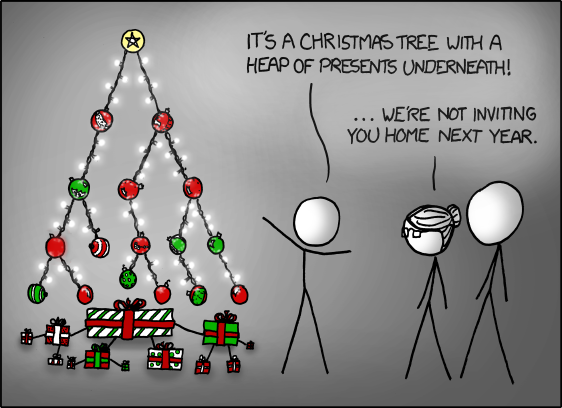
\includegraphics[scale=0.4]{tree.png}

\column{.3\textwidth}<2->
\vskip 24pt
Not only is that terrible in general, but you just KNOW Billy's going to open the root present first, and then everyone will have to wait while the heap is rebuilt.
\end{columns}

\end{frame}

